%%%%%%%%%%%%%%%%%%%%%%%%%%%%%%%%%%%%%%%%%%%%%%%%%%%%%%%%%%%%%%%%%%%%%%%%%%%%%%%%
%
% \chapter{Installation}\label{chInstallation}
%
%%%%%%%%%%%%%%%%%%%%%%%%%%%%%%%%%%%%%%%%%%%%%%%%%%%%%%%%%%%%%%%%%%%%%%%%%%%%%%%%

This chapter is a step-by-step guide on how to install the graphical user interface GiD, the finite element computational tool ERMES 20.0 and the external solver library PETSc.

\section{Graphical user interface}

The recommended pre- and post- processor tool for ERMES 20.0 is GiD \cite{GiDWeb}. To install GiD, download the last version from \url{https://www.gidsimulation.com} and follow the instructions provided on that same webpage. After finishing the installation, open GiD, and click on the upper menu: \textbf{\underline{H}elp} $\rightarrow$ \textbf{Register GiD}, as shown in Figure \ref{GiD-RegisterMenu}:
\\
\begin{figure}[!h]
	\begin{center}
		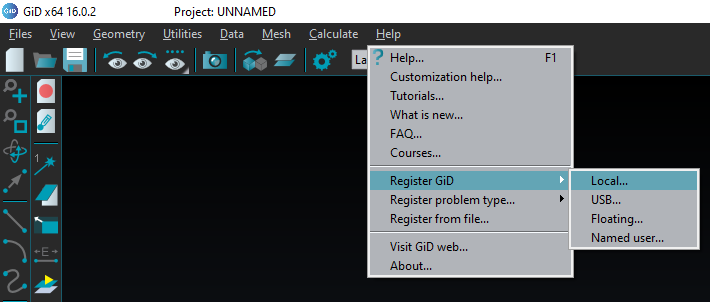
\includegraphics[width=0.95\textwidth]{Contents/Figures/GiD-RegisterMenu.png}
		\caption{Register GiD drop-down menu.}\label{GiD-RegisterMenu}
	\end{center}
\end{figure}
\\
Select \textbf{Local...} to register the local computer, \textbf{USB...} to register a USB stick attached to the local computer, \textbf{Floating...} to register a local network, or \textbf{Named user...} to attach the license to an email account. After clicking one of these options, a new window will appear with information related to the method selected and a link to obtain the password for a full professional license. Follow the link to get a one month free password or a permanent licence. The one month free license can be renewed up to three times for the same computer, USB stick, or email account. If the registration has been successful, the icon on the upper right corner of GiD will change colour as shown in Figure \ref{GiD-RegisterIcon}:
\\
\begin{figure}[!h]
\begin{center}

\includegraphics[width=0.5\textwidth]{Contents/Figures/GiD-RegisterButton.png}
\caption{GiD upper right icon indicating a successful registration.}\label{GiD-RegisterIcon}
\end{center}
\end{figure}

If a different pre- and post- processor software is preferred, the input files required by ERMES 20.0, and the output files it generates, can be edited and customized to meet the needs of any other pre- and post- processor tool (see Chapters \ref{chPreProcess} and \ref{chPostProcess} for a description of these input and output files).  

\section{ERMES 20.0}

If GiD is the chosen pre- and post- processor, the installation of ERMES 20.0 is very simple. The folder \path{\ERMES_20.0.5} is a problemtype of GiD. Therefore, the installation process consists in \textit{Copy\&Paste} the whole folder \path{\ERMES_20.0.5} inside the \path{\problemtypes} folder of GiD (located, for instance, in \path{C:\MySoftware\GiD 16.0.2\problemtypes}). The same installation process applies to Windows and Linux. 

To check that the installation has been done correctly, re-start GiD, and click on the GiD upper menu: \textbf{\underline{D}ata} $\rightarrow$ \textbf{Problem type}. ERMES 20.0 must appear in the drop-down menu as shown in Figure \ref{ERMES-Dopdrown}:

\begin{figure}[H]
	\begin{center}
		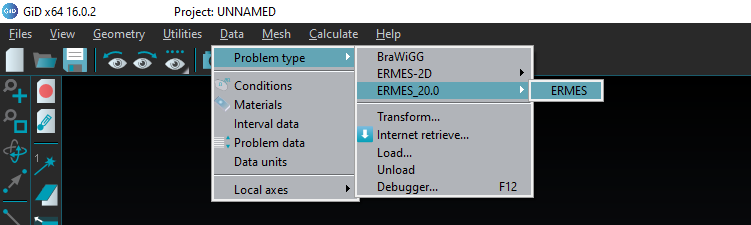
\includegraphics[width=\textwidth]{Contents/Figures/GiD-ERMES-Dropdown.png}
		\caption{GiD \textbf{\underline{D}ata} $\rightarrow$ \textbf{Problem type} drop-down menu showing ERMES 20.0 problemtype. Click on the ERMES submenu \textbf{\underline{D}ata} $\rightarrow$ \textbf{Problem type} $\rightarrow$ \textbf{ERMES\_20.0} $\rightarrow$ \textbf{ERMES} to start ERMES 20.0.}\label{ERMES-Dopdrown}
	\end{center}
\end{figure}

Click on the ERMES submenu \textbf{\underline{D}ata} $\rightarrow$ \textbf{Problem type} $\rightarrow$ \textbf{ERMES\_20.0} $\rightarrow$ \textbf{ERMES}. The ERMES logo and menu bar should appear, as shown in Figure \ref{ERMES-Start}, indicating that ERMES 20.0 has been successfully installed.

\begin{figure}[H]
	\begin{center}
		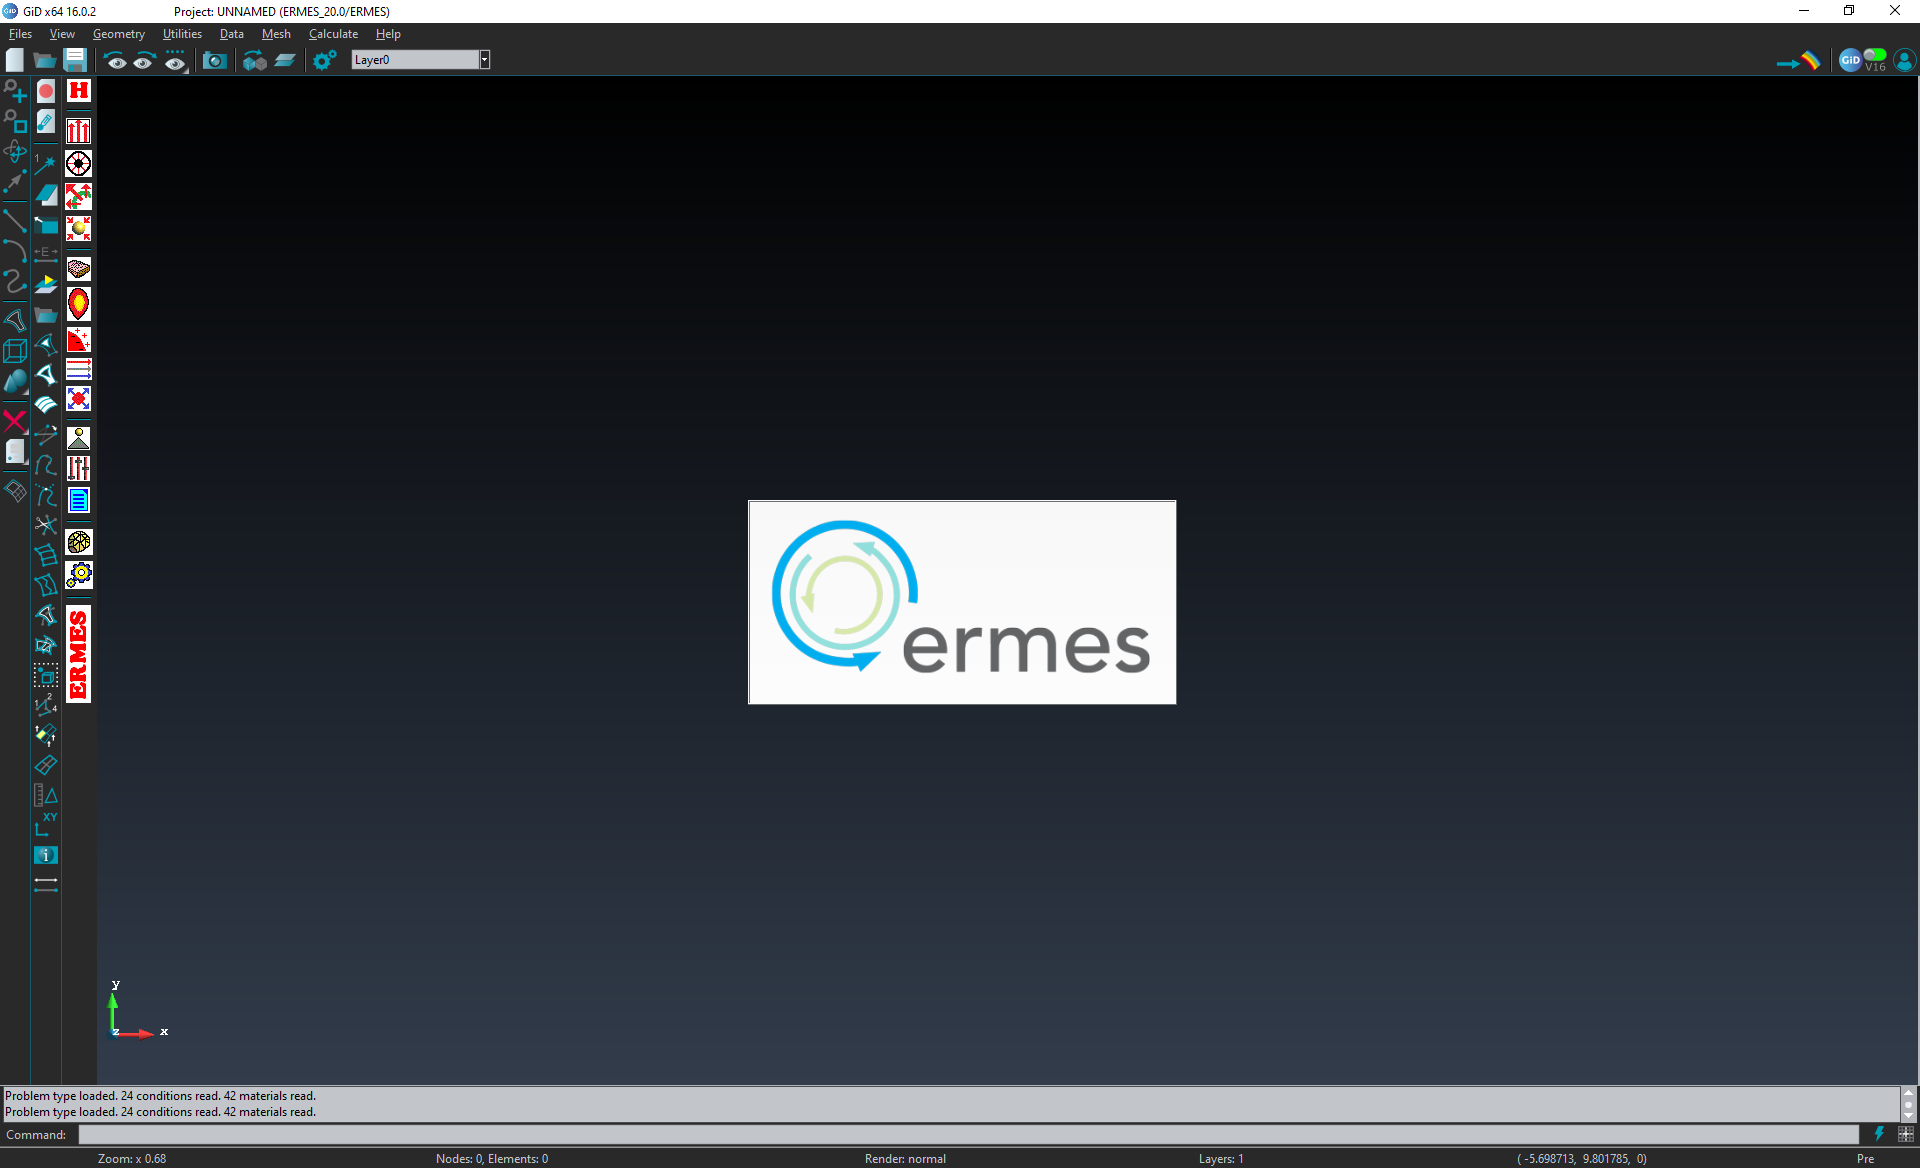
\includegraphics[width=0.96\textwidth]{Contents/Figures/ERMES-Start.png}
		\caption{ERMES 20.0 starting logo and menu bar.}\label{ERMES-Start}
	\end{center}
\end{figure}

If you open a GiD problem created with an earlier version of ERMES, you can upgrade it to a newer version (e.g., ERMES 20.0.5) by selecting ERMES 20.0.5 from the submenu above and choosing \textbf{Transform to new problem type}. When the differences between versions are significant, select \textbf{Reset to new problem type} to ensure that all fields are updated accordingly.

The executables included in the problem type are ready to run and do not require any additional installation: \path{\ERMES_20.0.5\ERMES.gid\execs\win\ERMES_20.0.5.exe} runs on any 64-bit Windows computer (together with the OpenMP runtime \path{vcomp140.dll} located in the same folder), and \path{\ERMES_20.0.5\ERMES.gid\execs\unix\ERMES_20.0.5} is statically linked and runs on any 64-bit x86 Linux computer, including HPC clusters. If the ERMES 20.0.5 C++ source code needs to be recompiled for any reason (e.g., because it has been modified to add a new feature), follow the instructions in \path{\ERMES_CPP_20.0.5\windows\README.txt} to compile ERMES for Windows, and the instructions in \path{\ERMES_CPP_20.0.5\unix\README.txt} to compile ERMES for Linux.

If the ERMES C++ source code is recompiled, verify that the ERMES version called by the \path{ERMES.unix.bat} script for Linux or the \path{ERMES.win.bat} script for Windows matches the version you intend to use. These scripts, located in the GiD problem type folder \path{\ERMES_20.0.5\ERMES.gid}, are responsible for launching ERMES when the \textit{Calculate} button is clicked in GiD. They can also be modified to include additional program calls, delete files, or perform other custom tasks. For Linux systems, ensure that execution permissions are granted to the script \path{ERMES.unix.bat} and any executables it references. 

\section{PETSc solvers library}\label{ExternalSolversInstall}

ERMES includes two iterative solvers, the biconjugate gradient (BiCG) and quasi-minimal residual (QMR) methods, both with diagonal preconditioning and OpenMP parallelization. These solvers have a low memory footprint and are highly efficient for well-conditioned matrices, but they may be insufficient for large, ill-conditioned linear systems. ERMES 20.0.5 also includes a direct solver, which can be used effectively on shared-memory computers when the iterative solvers struggle to converge.

For large, complex linear systems, we recommend the PETSc library \cite{PETScWeb}, which provides access to direct and iterative solvers, a wide range of preconditioning options, and MPI parallelization. PETSc can be installed on both Windows and Linux. However, we recommend installing it on Linux or, if Windows is required, running it through the Windows Subsystem for Linux (WSL).

The folder \path{\External_Solvers\PETSc_Solvers} within the problemtype directory contains the files required to call and execute PETSc, as well as a \path{README.txt} file with installation instructions and troubleshooting information. Follow the instructions in this \path{README.txt} to install and configure PETSc.

If a different solver library is preferred (e.g., Python NumPy \cite{NumPyWeb}), refer to the Python scripts in \path{\External_Solvers\NumPy_Solvers} for examples of how to read the linear system generated by ERMES 20.0, convert the matrix and vectors into different formats, and solve the system.